\documentclass[11pt,ngerman,a4paper]{article}
%Gummi|061|=)
\usepackage{amsmath}
\usepackage{a4wide}
\usepackage{amsthm}
\usepackage{url}
\usepackage{amsbsy}
\usepackage{amssymb}
\usepackage{inputenc}
\usepackage{graphicx}
\usepackage{rotating} 
\usepackage[separate-uncertainty=true]{siunitx}
\usepackage{booktabs}
\usepackage{paralist}
\usepackage{selinput}
\SelectInputMappings{%
adieresis={ä},
germandbls={ß},
}
\title{\textbf{Versuch V355: Gekoppelte Schwingkreise}}
\author{Martin Bieker\\
		Julian Surmann\\
		\\
		Durchgef\"{u}hrt am 09.01.2014\\
		TU Dortmund}
\date{}
\usepackage{graphicx}
\begin{document}
\renewcommand\tablename{Tabelle}
\renewcommand\figurename{Abbildung}
\maketitle
\thispagestyle{empty}
\newpage
\clearpage
\setcounter{page}{1}


\section{Einleitung}
Im folgenden Versuch sollen gekoppelte Oszillatoren untersucht werden. Bei diesen Systemen handelt es sich um schwingfähige Systeme, welche miteinander in Wechselwirkung stehen und so Energie austauschen können. 

\section{Theorie}

In diesem Versuch sollen zwei Schwingkreise untersucht werden, die über eine gemeinsame Koppelkapazität $C_K$ miteinander wechselwirken. Mit Hilfe der Kirchhoffschen Gesetze kann gezeigt werden, dass der Verlauf der Ströme $I_1$ und $I_2$ durch zwei gekoppelte Differentialgleichungen zweiter Ordnung bestimmt wird. Daraus folgt, dass $I_1$ und $I_2$ durch eine Überlagerung von zwei so genannten Fundamentalschwingungen beschreiben werden können. Diese haben die Frequenzen

\begin{equation}
\nu^+ = \frac{1}{2 \pi \sqrt{LC}}
\label{nueplus}
\end{equation}
und 
\begin{equation}
\nu^- =\frac1{2\pi\sqrt{L(\frac1C + \frac2{C_K})^-1}}.
\label{nueminus}
\end{equation}
Da die Werte von $L$, $C$ und $C_K$ mit Messunsicherheiten behaftet sind, müssen, um einen Vergleich von Theorie und Experiment zu ermöglichen, die Gesamtfehler dieser Größen bekannt sein. Diese wurden im Folgenden mit Hilfe der Fehlerfortpflanzung nach \textsc{Gauss} berechnet:

\begin{equation}
\Delta \nu_+ = \sqrt{\frac{\sigma_{L}^{2}}{16 \pi^{2} C L^{3}} + \frac{\sigma_{C}^{2}}{16 \pi^{2} C^{3} L}}
\end{equation}

\begin{equation}
\Delta \nu_- = \sqrt{\frac{\sigma_{L}^{2} \left(- \frac{1}{C_{K}} - \frac{1}{2 C}\right)^{2}}{4 \pi^{2} \left(L \left(\frac{2}{C_{K}} + \frac{1}{C}\right) - 1\right)^{3}} + \frac{L^{2} \sigma_{C_{K}}^{2}}{4 \pi^{2} C_{K}^{4} \left(L \left(\frac{2}{C_{K}} + \frac{1}{C}\right) - 1\right)^{3}} + \frac{L^{2} \sigma_{C}^{2}}{16 \pi^{2} C^{4} \left(L \left(\frac{2}{C_{K}} + \frac{1}{C}\right) - 1\right)^{3}}}
\end{equation}

\noindent

Im Folgenden soll der Stromverlauf für die Anfangsbedingungen

\[
I_1(0) = I_0 \neq 0
\] 
und 
\[
I_2(0) = 0
\]
untersucht werden. Zusätzlich wird angenommen, dass sich die Frequenzen $\nu_+$  und $\nu_-$ nur geringfügig unterscheiden. Den in diesem Fall auftretenden Schwingungsvorgang bezeichnet man als Schwebung. Dabei schwingen die Einzelkreise ungefähr mit der Frequenz $\nu_+$. Des Weiteren ändert sich die Amplitude der Schwingung mit der wesentlich geringeren Frequenz 
\begin{equation}
\nu_{Schwebung} = \nu_- - \nu_+.
\end{equation}

\section{Aufbau und Durchf\"{u}hrung}
\subsection{Vorbereitungen}
Vor Beginn der Messungen müssen die Resonanzfrequenzen beider Schwinkreise aufeinander abgestimmt werden. Dazu wird die Schaltung wie in Abbildung \ref{abb1} gezeigt aufgebaut.
\begin{figure}[htp]
\centering
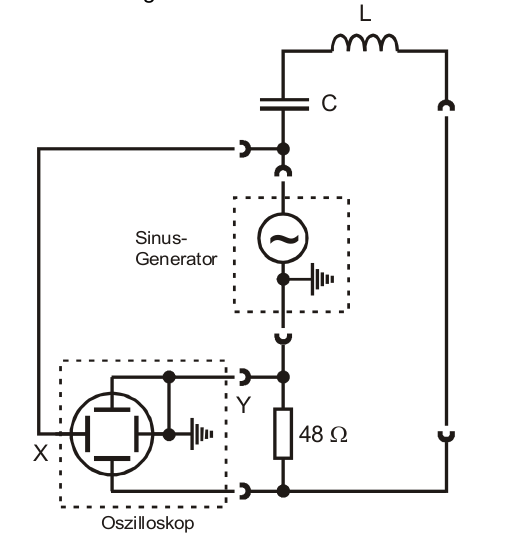
\includegraphics[scale=0.5]{Abb/abb1.png}
\caption{Diese Schaltung dient zum Kalibrieren der Resonanzfrequenzen beider Schwingkreise. [1]}
\label{abb1}
\end{figure}
In einem der Kreise ist ein Kondensator mit variabler Kapazität verbaut. Mit dem Sinusgenerator wird nun der Kreis mit konstanter Kapazi\"at angeregt. Zunächst wird mit dem Oszilloskop im YT-Betrieb die Frequenz ermittelt, bei der die gemessene Spannung $U_R$ maximal wird. Dann wird das Oszilloskop in den XY-Modus umgeschaltet die Resonanzfrequnz $\nu_{res}$ bestimmt. Diese zeichnet sich dadurch aus, dass $U_R$ und die Generatorspannung $U_0$ in Phase liegen und daher die angezeigte Lissajous-Figur eine Gerade ist. Danach wird der Sinusgenerator an den zweiten Teil des Schwingkreises angeschlossen und mit der Frequenz $\nu_{res}$ angeregt. Nun wird auch dieser Kreis durch Veränderung der variablen Kapazität in Resonanz gebracht. Dazu werden wie zuvor Lissajous-Figuren verwendet. 
\subsection{Messung vom Schwebungs- und Schwingungsfrquenz}
Für diesen Versuchsteil wird die Schaltung wie in Abbildung \ref{abb2} aufgebaut.
\begin{figure}[h!]
\centering
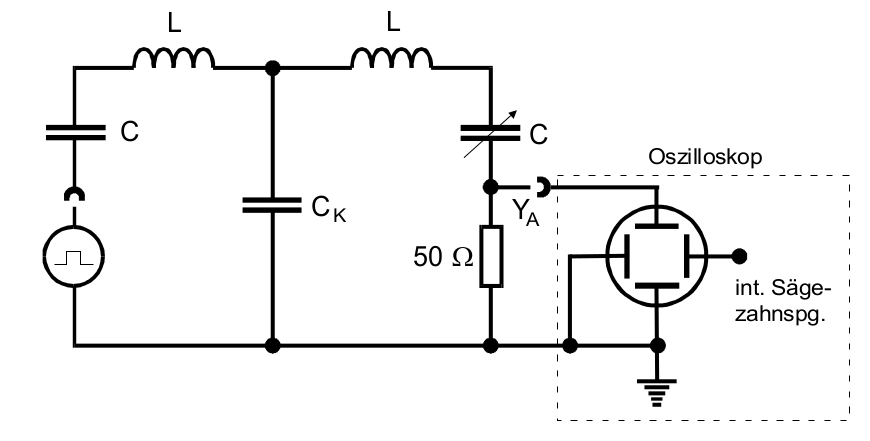
\includegraphics[scale=0.5]{Abb/abb2.png}
\caption{Diese Schaltung dient zur Messung des Verhältnisses von Schwebungs- zu Schwingungfrequenz. [2] }
\label{abb2}
\end{figure}
Der linke Schwingkreis wird durch eine Rechteckspannung zu Schwingungen angeregt. Mit dem Oszilloskop wird nun die am Widerstand $R$ abfallende Spannung gemessen. So kann der im rechten Schwingkreis fließende Strom bestimmt werden. Bei verschiedenen Koppelkapazitäten $C_K$ wird nun das Verhältnis von Schwingungs- und Schwebungsfrequenz bestimmt. Dazu wird die Zahl $n$ der Schwingungsmaxima in einer Schwebungsperiode ermittelt. Es gilt:
\begin{equation}
\frac{\nu_{Schwingung}}{\nu_{Schwebung}} = n
\end{equation}
\subsection{Messung der Frequenzen der Fundamentalschwingungen}
Des Weiteren sollen die Frequenzen $\nu_-$ und $\nu_+$ bestimmt werden. Diese zeichen sich dadurch aus, dass die Phasenverschiebung zwischen der Erregerspannung und dem im Sekundärkreis fließenden Stroms $0$ oder $\pi$ beträgt. Die oben verwendete Schaltung wird nun mit einer Sinusspannung angeregt und das Generatorsignal auf den zweiten Kanal des Oszilloskops gelegt (siehe Abb. \ref{abb3}).
\begin{figure}[h!]
\centering
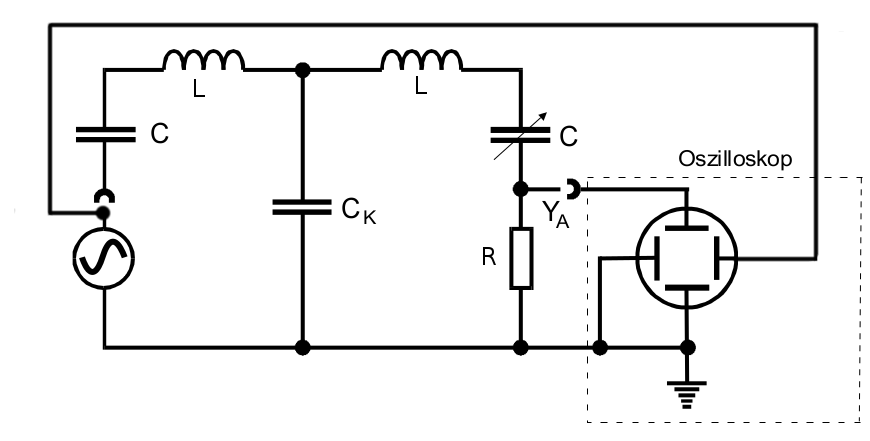
\includegraphics[scale=0.5]{Abb/abb3.png}
\caption{Diese Schaltung dient  zur Messung der Frequenzen der Fundamentalschwingungen. [2]}
\label{abb3}
\end{figure}
So kann die Phasenbeziehung von $I$ und $U_0$ mit Hilfe von Lissajous-Figuren untersucht werden. So werden $\nu_+$ und $\nu_-$ in Abhängikeit von $C_K$ bestimmt.
\subsection{Messung des Stroms in Abhängigkeit von der Erregerfrequenz}

Um den Verlauf des Stroms $I$ im Sekundärkreis bei in Abhängigkeit von der Erregerfrequenz darzustellen, wird die Schaltung wie in Abbildung \ref{abb1} aufgebaut. Mit dem Unterschied, dass der Funktionsgenerator im Sweep-Betreib arbeitet. Dies bedeutet, dass die Frequenz der Erregerspannung nicht mehr konstant ist, sondern steigt in der Zeit $\Delta t =\SI{21}{\milli\second}$ von $\nu_0 = \SI{3,8}{\kilo\hertz}$ auf $\nu_1 = \SI{74,2}{\kilo\hertz}$. Mit der Verlauf der am Widerstand abfallenden Spannung gemessen werden. Dabei wird die Zeitbasis des Oszilloskops so eingestellt, dass ein vollständiger Sweep auf dem Schirm zu sehen ist. Anfang und Ende dieses Zyklus entsprechen den Frequenzen $\nu_0$ und $\nu_1$.     



\section{Auswertung}


Sofern nicht anders angegeben, wurden alle Fehler mit python uncertainties berechnet.
\subsection{Vorbereitungen}
Für die Justierung des Messaufbaus wurde mit der Grobmessung eine Frequenz von \SI{30,69+-0,01}{\kilo\hertz} ermittelt. Die feine Messung mit Hilfe der Lissajous-Figuren ergab eine Resonanzfrequenz von $\SI{30,70+-0,01}{\kilo\hertz}$. Der mit L und C theoretisch berechnete Wert liegt bei \SI{30,49}{\kilo\hertz}, mit einer Abweichung von \SI{0,68}{\percent} ausgezeichnet im Toleranzbereich. Allerdings wurde in der Berechnung des theoretischen Wertes die Kapazität der Spule schon berücksichtigt.
\subsection{Messung von Schwebungs- und Schwingungsfrequenz}
Die Perioden pro Schwebungsperiode wurden so genau wie möglich abgelesen. Der Fehler liegt bei maximal $\pm 0.5$ Perioden. Diese Werte sind der Tabelle 1 zu entnehmen. Der bei $C_K$ angegebene Fehler ist ein auf die Werte umgerechneter Fehler von $\pm 3 \%$. Dieser ist an der Messapparatur vorgegeben.

\noindent
Die Frequenz $\nu_{theo}^+$ ist konstant und beträgt \SI{30,493}{\kHz}. Diese wurde mit Formel \ref{nueplus} berechnet.  $\nu_{theo}^-$ wurde mit Formel \ref{nueminus} ermittelt. Der Mittelwert der beiden Frequenzen wurde mit 
\[
\overline{\nu}=\frac{1}{2}(\nu_-+\nu_+)
\]
ermittelt. Die Frequenz der Schwebung ist durch $\nu_{theo}^--\nu_{theo}^+$ gegeben. Diese theoretisch ermittelten Werte befinden sich in Tabelle 2. Abbildung \ref{41} zeigt sowohl das experimentell ermittelte, als auch das berechnete Frequenzverhältnis in Abhängigkeit von der verwendeten Koppelkapazität.
\begin{figure}[h]
\centering
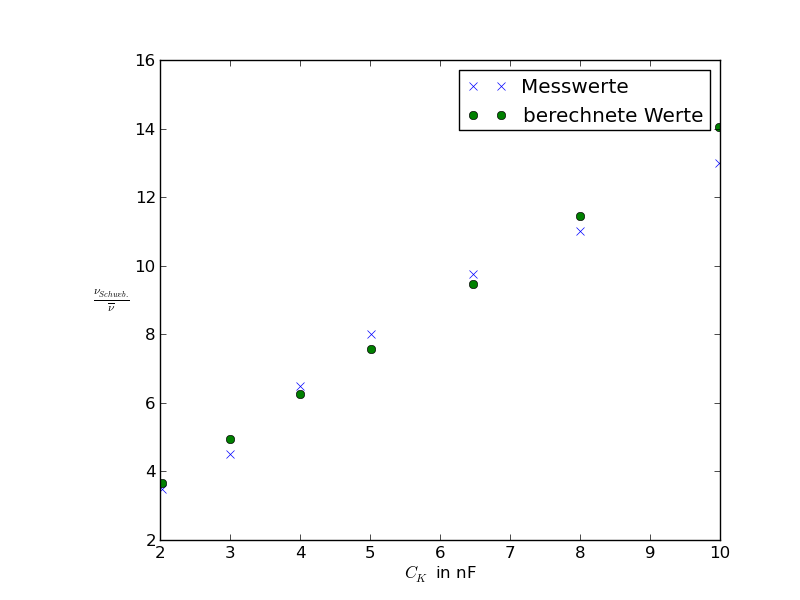
\includegraphics[scale=0.6]{Abb/diag1.png}
\caption{Diese Abbildung zeigt das Verhältnis von Schwebungs- zu Schwingungsfrequenz für verschiedene Koppelkapazitäten}
\label{41}
\end{figure}

\noindent
Die in der Tabelle 3 angebebene Abweichung bezieht sich auf den Unterschied vom experimentellen zum theoretischen Frequenzverhältnis.
\subsection{Messung der Frequenzen der Fundamentalschwingungen}
Für die Messung der Frequenzen wurden Lissajous-Figuren benutzt. Die Frequenzen $\nu_+$ und $\nu_-$ wurden aufgenommen als die Generatorspannung und der Strom im Sekundärkreis jeweils gleich- oder gegenphasig verlaufen. Die Frequenzen werden in Tabelle 4 mit den Theoriewerten aus 4.2 Verglichen. Dies ist auch in den Abbildungen \ref{42} und \ref{43} dargestellt. Diese zeigen den Verlauf von $\nu_+$ und $\nu_-$ in Abhängigkeit von der verwendeten Koppelkapazität $C_K$ dar.
\begin{figure}[h!]
\centering
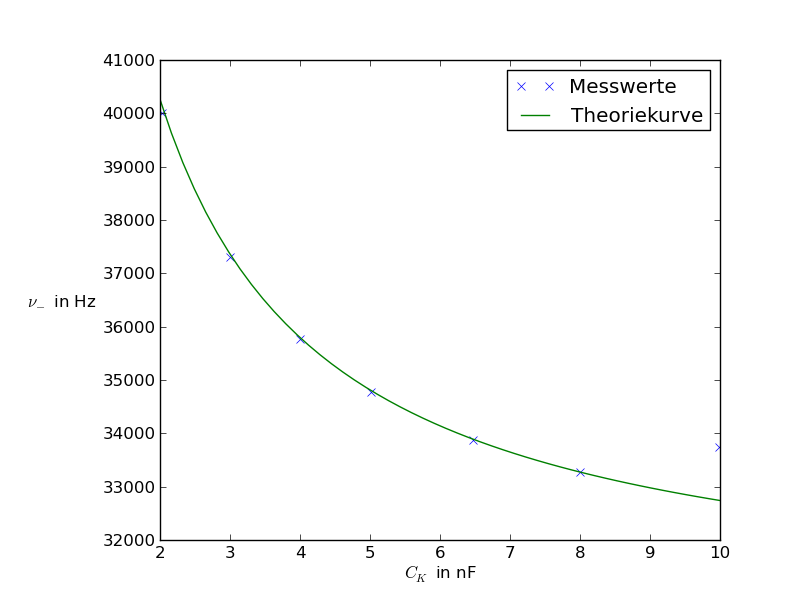
\includegraphics[scale=0.6]{Abb/diag2.png}
\label{42}
\caption{Diese Grafik zeigt die Frequenz $\nu_-$ für verschiedene Werte von $C_K$.}
\end{figure}
\begin{figure}[h!]
\centering
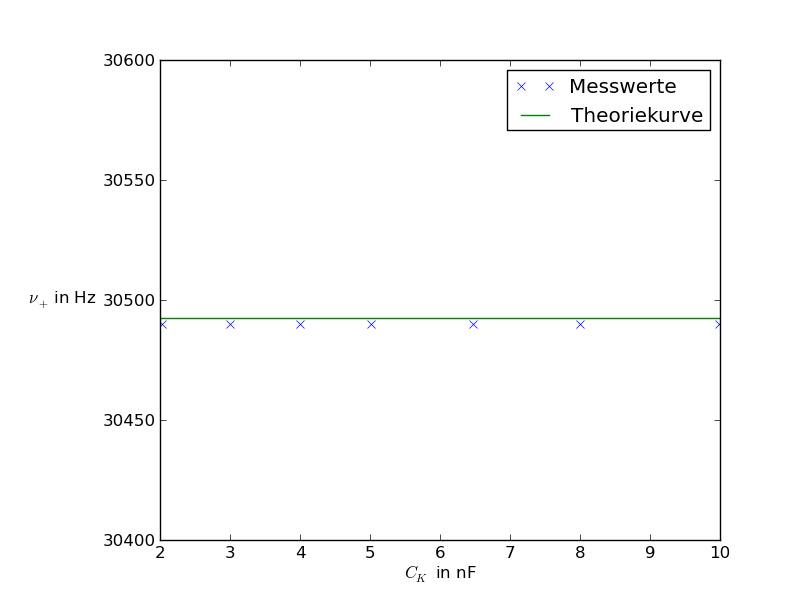
\includegraphics[scale=0.6]{Abb/diag3.png}
\caption{Diese Grafik zeigt die Frequenz $\nu_+$ für verschiedene Werte von $C_K$.}
\label{43}
\end{figure}
\noindent
Die Berechnungen zeigen eine Abweichung vom Theoriewert von jeweils ca. \SI{1}{\percent}.
\subsection{Messung des Stroms in Abhängigkeit von der Erregerfrequenz}
Die in dieser Messreihe aufgenommenen Werte sind in Tabelle 5 ersichlich.
Die bei den zeitlichen Abständen und der Spannung angegebenen Unsicherheiten entsprechen der Hälfte der kleinsten angezeigten Skaleneinteilungen des Oszilloskops. Aus den zeitlichen Abständen $d_1$ und $d_2$ kann mit folgenden Zusammenhängen die zugehörige Frequenz berechnet werden:
\begin{itemize}
\item $f_1 = \left( \frac{70400\cdot d_1}{\SI{21}{\milli\second}}+3800 \right)\si{\Hz}$
\item $f_2 = \left( \frac{70400\cdot d_2}{\SI{21}{\milli\second}}+3800\right)\si{\Hz}$.
\end{itemize}
Diese sind in Tabelle 6 angegeben. Die Ströme wurden mit dem Ohmschen Gesetz berechnet. Allerdings wurde der Widerstand mit \SI{73}{\ohm}  statt mit \SI{48}{\ohm} angenommen, da weitere Dämpfungseffekte zum Beispiel durch die in den Stromkreisen vorhandenen Spulen auftreten. Für die verschiedenen untersuchten Koppelkapazitäten wurden die jeweils gemessenen Ströme $I_1$ und $I_2$ in Abbildung \ref{44} aufgetragen.
\begin{figure}[h]
\centering
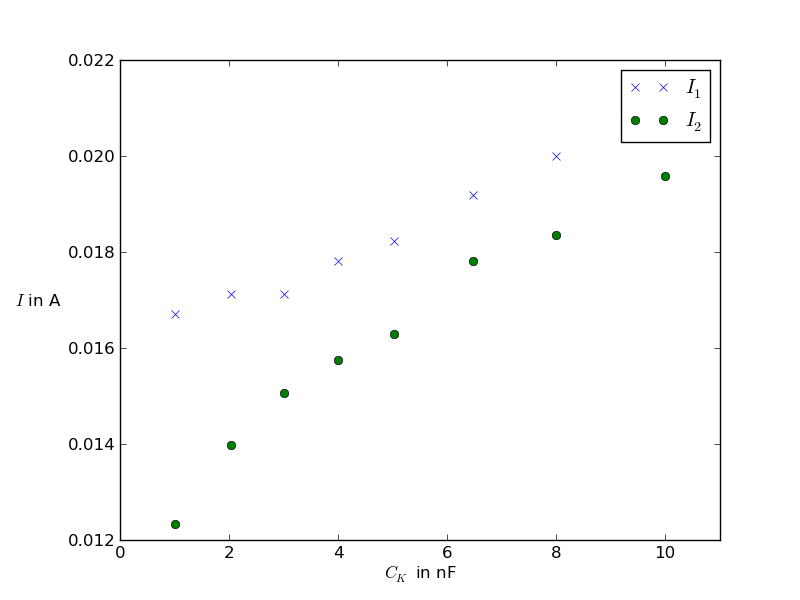
\includegraphics[scale=0.6]{Abb/diag4.png}
\caption{Diese Grafik zeigt den Verlauf der Ströme $I_1$ und $I_2$ für verschiedene Werte von $C_K$.}
\label{44}
\end{figure}

\section{Diskussion}
Insgesamt sind alle Unsicherheiten innerhalb der üblichen Toleranzen. Die Messfehler beim Ablesen der Werte auf dem Bildschirm des Oszilloskopes wurden eher pessimistisch angenommen, sie sind auf jeden Fall groß genug angenommen. Die Abweichungen der experimentellen zu den theoretischen Frequenzen sind mit $<$ 10 \% tolerierbar.\newline
In den anderen Versuchsteilen sind die Abweichungen alle gering.

\section{Literatur- und Abbildungsverzeichnis}
\begin{enumerate}[{[}1{]}]
\item Entnommen aus: \\\textit{Versuch Nr.355 Gekoppelte Schwingkreise}, TU Dortmund\\
Download am 09.01.14 unter:\\
\url{http://129.217.224.2/HOMEPAGE/PHYSIKER/BACHELOR/AP/SKRIPT/V355.pdf}
\item Geringfügig bearbeitete Grafiken aus:\\ \textit{Versuch Nr.355 Gekoppelte Schwingkreise}, TU Dortmund\\
Download am 09.01.14 unter:\\
\url{http://129.217.224.2/HOMEPAGE/PHYSIKER/BACHELOR/AP/SKRIPT/V355.pdf}
\end{enumerate}
\section{Anhang}
\begin{itemize}
\item Auszug aus dem Messheft
\end{itemize}

\newpage
\begin{table}[h]

\label{tab1}
\centering
\begin{tabular}{SSS}
\toprule
{n} &{ $\frac{C_K}{\si{\nano\farad}}$} &{ Frequenzverh\"altnis }\\
\midrule
1 & 12.03(6) & 3.5(5)  \\
2 & 23.00(9) & 4.5(5)  \\
3 & 34.00(12) & 6.5(5)  \\
4 & 45.02(15) & 8.0(5)  \\
5 & 56.47(19) & 9.8(5)  \\
6 & 68.00(24) & 11.0(5)  \\
7 & 79.99(30) & 13.0(5)  \\
\bottomrule
\end{tabular}

\caption{Diese Tabelle zeigt das ermittelte Frequenzverh\"altnis in Abh\"angigkeit von der Koppelkapazit\"at.}



\begin{tabular}{llll}
\toprule
{n} &{$\frac{\overline{f}}{\si{\Hz}}$} &{$\frac{f_{Schweb.-th.}}{\si{\Hz}}$} &{ th. Frequenzverh\"altnis }\\
\midrule
1 & $\left(3.532 \pm 0.013\right) \times 10^{4}$  & $\left(9.65 \pm 0.25\right) \times 10^{3}$  & $3.66 \pm 0.08$ \\
2 & $\left(3.393 \pm 0.010\right) \times 10^{4}$  & $\left(6.87 \pm 0.18\right) \times 10^{3}$  & $4.94 \pm 0.12$ \\
3 & $\left(3.314 \pm 0.008\right) \times 10^{4}$  & $\left(5.30 \pm 0.14\right) \times 10^{3}$  & $6.25 \pm 0.16$ \\
4 & $\left(3.265 \pm 0.007\right) \times 10^{4}$  & $\left(4.31 \pm 0.12\right) \times 10^{3}$  & $7.58 \pm 0.20$ \\
5 & $\left(3.219 \pm 0.005\right) \times 10^{4}$  & $\left(3.40 \pm 0.10\right) \times 10^{3}$  & $9.47 \pm 0.25$ \\
6 & $\left(3.188 \pm 0.005\right) \times 10^{4}$  & $\left(2.78 \pm 0.08\right) \times 10^{3}$  & $11.46 \pm 0.31$ \\
7 & $\left(3.162 \pm 0.004\right) \times 10^{4}$  & $\left(2.25 \pm 0.06\right) \times 10^{3}$  & $14.10 \pm 0.40$ \\
\bottomrule
\end{tabular}
\label{tab2}
\caption{Diese Tabelle zeigt die berechneten Werte f\"ur Frequenzverh\"altnis und Schwebungsfrequenz.}


\begin{tabular}{llll}
\toprule
{n} &{exp. Freq.-Verh.} &{exp. Freq.-Verh.} &{$\frac{\Delta}{\si{\percent}}$}\\
\midrule
1 & $3.5 \pm 0.5$  & $3.66 \pm 0.08$  & 4 \\
2 & $4.5 \pm 0.5$  & $4.94 \pm 0.12$  & 4\\
3 & $6.5 \pm 0.5$  & $6.25 \pm 0.16$  & 4  \\
4 & $8.0 \pm 0.5$  & $7.58 \pm 0.20$  & 6 \\
5 & $9.8 \pm 0.5$  & $9.47 \pm 0.25$  & 3 \\
6 & $11.0 \pm 0.5$  & $11.46 \pm 0.31$ & 4 \\
7 & $13.0 \pm 0.5$  & $14.1 \pm 0.4$  & 7 \\
\bottomrule
\end{tabular}
\label{tab3}
\caption{In dieser Tabelle werden die experimentell gewonnenen Daten mit den rechnerisch ermittelten verglichen.}
 \end{table}
 
 \begin{table}
 \centering
\begin{tabular}{llllll}
\toprule
{$\frac{C_K}{\si{\Hz}}$} & {$\frac{\nu_{+th}}{\si{\Hz}}$} & $\frac{\nu_{+ex}}{\si{\Hz}}$ &$\frac{\nu_{+th}}{\si{\Hz}} $& $\frac{\Delta_{\nu+}}{\si{\percent}}$ &$\frac{\Delta_{\nu-}}{\si{\percent}}$\\
\midrule
 $1.010 \pm 0.030$  & $\left(4.014 \pm 0.025\right) \times 10^{4}$  & 30490 & 40010 & 1.0 & 0.997\\
 $2.03 \pm 0.06$  & $\left(3.736 \pm 0.019\right) \times 10^{4}$  & 30490 & 37300 & 1.0 & 0.998\\
 $3.00 \pm 0.09$  & $\left(3.580 \pm 0.015\right) \times 10^{4}$  & 30490 & 35760 & 1.0 & 0.999\\
 $4.00 \pm 0.12$  & $\left(3.480 \pm 0.012\right) \times 10^{4}$  & 30490 & 34780 & 1.0 & 0.999\\
 $5.02 \pm 0.15$  & $\left(3.389 \pm 0.010\right) \times 10^{4}$  & 30490 & 33880 & 1.0 & 1.0\\
 $6.47 \pm 0.19$  & $\left(3.327 \pm 0.008\right) \times 10^{4}$  & 30490 & 33280 & 1.0 & 1.0\\
 $8.00 \pm 0.24$  & $\left(3.274 \pm 0.007\right) \times 10^{4}$  & 30490 & 33750 & 1.0 & 1.031\\
\bottomrule
\end{tabular}
\label{tab4}
\caption{Diese Tabelle zeigt die gemessen Frequenzen der Fundamentalschwingungen.}

\centering
\begin{tabular}{lllll}
\toprule
{$\frac{C_K}{\si{\nano\farad}}$} &{ $\frac{t_1}{\si{\milli\second}}$} &{ $\frac{t_1}{\si{\milli\second}}$} &{ $\frac{U_1}{\si{\volt}}$} &{ $\frac{U_2}{\si{\volt}}$ }\\
\midrule
 $1.010 \pm 0.030$  & $9.0 \pm 0.5$  & $13.7 \pm 0.5$  & $1.22 \pm 0.05$  & $0.90 \pm 0.05$ \\
 $2.03 \pm 0.06$  & $9.0 \pm 0.5$  & $11.8 \pm 0.5$  & $1.25 \pm 0.05$  & $1.02 \pm 0.05$ \\
 $3.00 \pm 0.09$  & $9.0 \pm 0.5$  & $10.9 \pm 0.5$  & $1.25 \pm 0.05$  & $1.10 \pm 0.05$ \\
 $4.00 \pm 0.12$  & $9.0 \pm 0.5$  & $10.5 \pm 0.5$  & $1.30 \pm 0.05$  & $1.15 \pm 0.05$ \\
 $5.02 \pm 0.15$  & $9.0 \pm 0.5$  & $10.1 \pm 0.5$  & $1.33 \pm 0.05$  & $1.19 \pm 0.05$ \\
 $6.47 \pm 0.19$  & $9.0 \pm 0.5$  & $9.9 \pm 0.5$  & $1.40 \pm 0.05$  & $1.30 \pm 0.05$ \\
 $8.00 \pm 0.24$  & $9.0 \pm 0.5$  & $9.5 \pm 0.5$  & $1.46 \pm 0.05$  & $1.34 \pm 0.05$ \\
 $9.99 \pm 0.30$  & $9.0 \pm 0.5$  & $9.5 \pm 0.5$  & $1.55 \pm 0.05$  & $1.43 \pm 0.05$ \\
\bottomrule
\end{tabular}
\label{tab5}
\caption{}

\centering
\begin{tabular}{lllll}
\toprule
{$\frac{C_K}{\si{\nano\farad}}$} &{ $\frac{\nu_1}{10\si{\kilo\Hz}}$} &{ $\frac{\nu_2}{10\si{\kilo\Hz}ß}$} &{ $\frac{I_1}{\si{\ampere}}$} &{ $\frac{I_2}{\si{\ampere}}$ }\\
\midrule
 $1.010 \pm 0.030$  & $3.40 \pm 0.17$   & $4.97 \pm 0.17$  & $0.0167 \pm 0.0007$  & $0.0123 \pm 0.0007$ \\
 $2.03 \pm 0.06$  & $3.40 \pm 0.17$  & $4.34 \pm 0.17$  & $0.0171 \pm 0.0007$  & $0.0140 \pm 0.0007$ \\
 $3.00 \pm 0.09$  & $3.40 \pm 0.17 $  & $4.03 \pm 0.17$  & $0.0171 \pm 0.0007$  & $0.0151 \pm 0.0007$ \\
 $4.00 \pm 0.12$  & $3.40 \pm 0.17 $  & $3.90 \pm 0.17$  & $0.0178 \pm 0.0007$  & $0.0158 \pm 0.0007$ \\
 $5.02 \pm 0.15$  & $3.40 \pm 0.17$  & $3.77 \pm 0.17$  & $0.0182 \pm 0.0007$  & $0.0163 \pm 0.0007$ \\
 $6.47 \pm 0.19$  & $3.40 \pm 0.17$  & $3.70 \pm 0.17$  & $0.0192 \pm 0.0007$  & $0.0178 \pm 0.0007$ \\
 $8.00 \pm 0.24$  & $3.40 \pm 0.17$  & $3.56 \pm 0.17$  & $0.0200 \pm 0.0007$  & $0.0184 \pm 0.0007$ \\
 $9.99 \pm 0.30$  & $3.40 \pm 0.17 $  & $3.56 \pm 0.17$  & $0.0212 \pm 0.0007$  & $0.0196 \pm 0.0007$ \\
\bottomrule
\end{tabular}
\label{}
\caption{}
\end{table}
\end{document}
